% \documentclass{jsarticle}
% \usepackage[dvipdfmx]{graphics}
% \usepackage{amsmath}
% \usepackage{amssymb}
% \usepackage{ascmac}
% \usepackage{bm}
% \usepackage{url}
% \usepackage{txfonts}
%
% \newcommand{\mmm}{\hspace{3mm}}
% \newcommand{\veczero}{$\vec{0}$}
% \newcommand{\veca}{$\vec{a}$}
% \newcommand{\vecb}{$\vec{b}$}
% \newcommand{\veco}{$\vec{o}$}
% \newcommand{\vecx}{$\vec{x}$}
% \newcommand{\vecy}{$\vec{y}$}
% \newcommand{\vecz}{$\vec{z}$}
%
%
%
%
% \begin{document}

    \section{ベクトルの定義}
    \subsection{教科書的理解}
    多くの教科書に"ベクトルとは,大きさと向きを持った量"という説明がある.図\ref{fig:vector_yukosenbun}のようなものだろう.矢印の長さが大きさを,さす方向が向きを表している.有向線分という表現も一度は目にしたことがあるだろう.
    %
    \begin{figure}[htbp]
        \begin{center}
            \resizebox{!}{4cm}{
            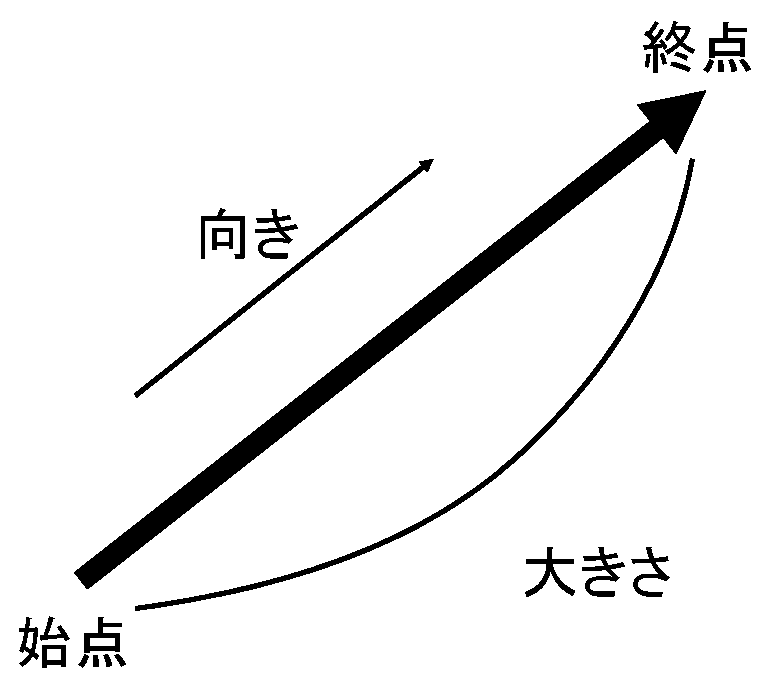
\includegraphics{img/vector_yukosenbun.eps}
            }
        \end{center}
        \caption{有向線分}
        \label{fig:vector_yukosenbun}
    \end{figure}

    今まで意識せずに扱ってきた数値というものは,向きのない大きさだけの量で"スカラ"と呼ばれる.計算では主にこのスカラ量を用いている.いや,計算で主にスカラ量を使っているのではなく,スカラ量であれば計算できるのだ.

    ベクトルの計算を考えたとき,その大きさを扱うのはそれほど難しくはないことが想像できる.これは大きさが数値,すなわちスカラ量であることが理由だ.では向きの計算はどうか.これが問題なのだ.向きといったものは数値として表現するのは簡単ではない.角度を使うことを考えることはできるが,これは数3において扱う極座標,さらには複素数平面で扱う事柄であってそこそこ難しい.

    ベクトルは向きのある量を扱う計算として,この計算が容易ではない"向き"という要素を上手に解決している.

    このような問題意識のもと,次へ進む.

    \subsection{2種のベクトル}
    すでに勉強したのであればベクトルと一口に言っても大きく2つの種類があったと思われる.まず1つ目に挙げられるのは
    \[
    \vec{a},\vec{b},\cdots
    \]
    というように矢印を頭にのせてベクトルを表現と,
    \[
    (1,0),(3,2),\cdots
    \]
    というようにあたかも座標のようにベクトルを表しているものである.この両者は先の問題意識として挙げた向きは計算できないという数学上の問題を解決している.

    ベクトルの問題を解く際にこの2つの違いは解答の方針に大きな差を生むので,同じベクトルの問題という一つのまとまりだという認識ではなく,$\vec{a},\cdots$を使うベクトルの問題,$(1,0),\cdots$を使うベクトルの問題,と分けて理解することを勧める.

    両者の独立した理解が,それらの併用という新たな選択肢を生む.両者の違いを意識して学習しよう.

    \section{$\vec{a}$のようなベクトル}
    文字に矢印をつけてベクトルを表現している.これは大きさ,向きの1セットを1つの記号$\vec{a}$であらわしている.しかし,その中身がどうなっているのかはわからないことが多い.まずは中身がわからなくとも計算が進められるように準備したい.

    \subsection{文字の計算の理解}
    話は一度ベクトルから離れる.中学,高校と算数が数学へとなってから,計算式には文字が登場するようになった.
    \[
    a+2b,\mmm (a+b)^2=a^2+2ab+b^2,\cdots
    \]
    このような文字の内容がわからなくても計算ができ,計算結果に何を代入しても正しいということである.例えば次の式を考える.
    \[
    a^3+ 3a^2b +3 ab^2 +b^3
    \]
    これに$a=3,b=-1$を代入して計算をすると
    \[
    a^3+ 3a^2b +3 ab^2 +b^3=8
    \]
    とわかる.これを
    \[
    a^3+ 3a^2b +3 ab^2 +b^3=(a+b)^3
    \]
    としても同様であろう.

    あまりに当然の話だ.いちいち読んでもらうのも申し訳ない.ここで述べたいのはそのようなことではない.今の説明では文字というのはスカラ量であった.これをベクトルという,大きさだけでなく向きを持った量で実現することができないかということだ.

    $\vec{a},\vec{b},\cdots$といったベクトルを表す文字に対しても普通の文字式が成立するようにしてゆく.

    \subsection{加算,減算}
    文字の計算の1つは足し算だ.$\vec{a},\vec{b}$の和を考える.これは容易で単純に足せばいい.
    \[
    \vec{a}+\vec{b}
    \]
    これを矢印であらわすと図\ref{fig:vector_tasizan}のようになる.矢印の始点と終点をつないでいる.
    %
    \begin{figure}[htbp]
        \begin{center}
            \resizebox{!}{4cm}{
            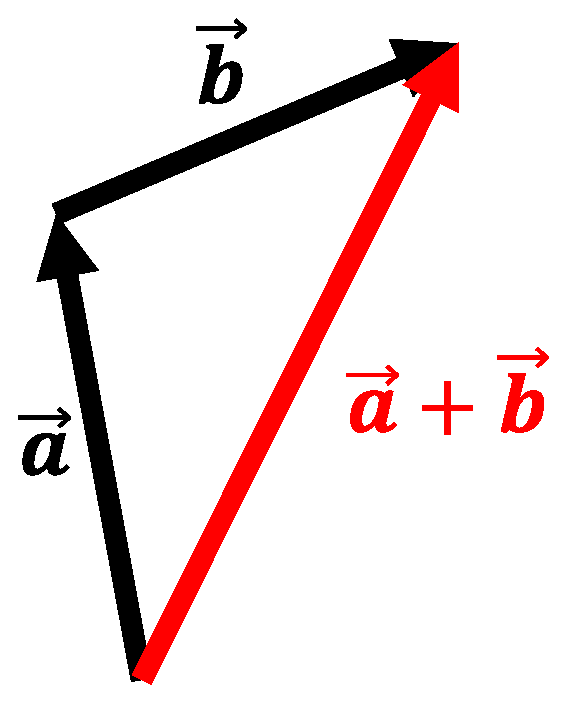
\includegraphics{img/vector_tasizan.eps}
            }
        \end{center}
        \caption{ベクトルの足し算}
        \label{fig:vector_tasizan}
    \end{figure}

    次は引き算だ.これも先と同様に
    \[
    \vec{a}-\vec{b}
    \]
    とすればよいが.これで十分な理解とは言えない.
    \[
    \vec{a}+ (-\vec{b})
    \]
    とすることでマイナスのベクトルを考えてみる.

    負の大きさというのが少しイメージしにくい\footnote{大きさは0以上の値をとる.絶対値の考えを使うからだ.}が結局のところ向きが逆\footnote{ベクトルは向きが存在するので,基本的には存在しない"負の大きさ"というものを考えることができる.向きを逆にするということで対処するのだ.}になる.図\ref{fig:vector_mainasu}のようなことだ.
    \begin{figure}[htbp]
        \begin{center}
            \resizebox{!}{3cm}{
            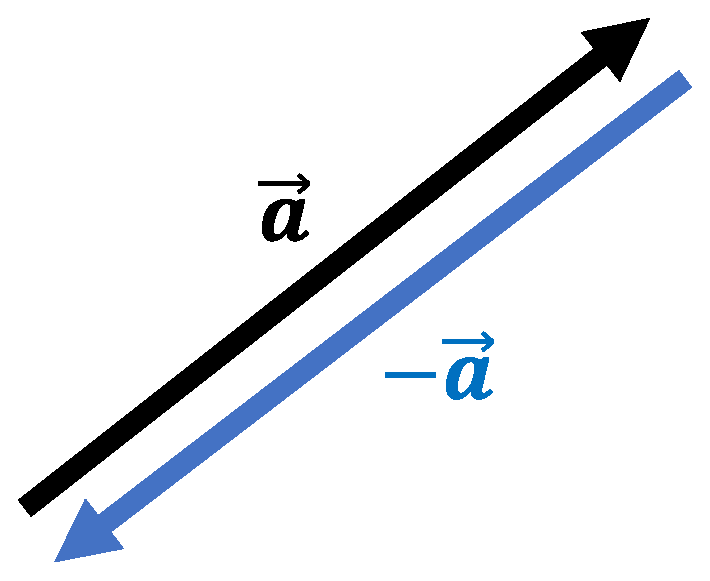
\includegraphics{img/vector_mainasu.eps}
            }
        \end{center}
        \caption{マイナスのベクトル}
        \label{fig:vector_mainasu}
    \end{figure}
    %

    マイナスのベクトルを導入したうえでベクトルの引き算を図示する.図\ref{fig:vector_hikizan1}のようになる.さらにマイナスのベクトルをもとに戻すと図\ref{fig:vector_hikizan2}のようになる.ここからベクトルの引き算は2つのベクトルの終点同士を引くベクトル(ここでは$\vec{b}$)から引かれるベクトル(ここでは$\vec{a}$)へつなげればいいことがわかる.
    %
    \begin{figure}[htbp]
        \begin{center}
            \begin{tabular}{c}

                \begin{minipage}{0.45\hsize}
                    \begin{center}
                        \resizebox{0.7\hsize}{!}{
                        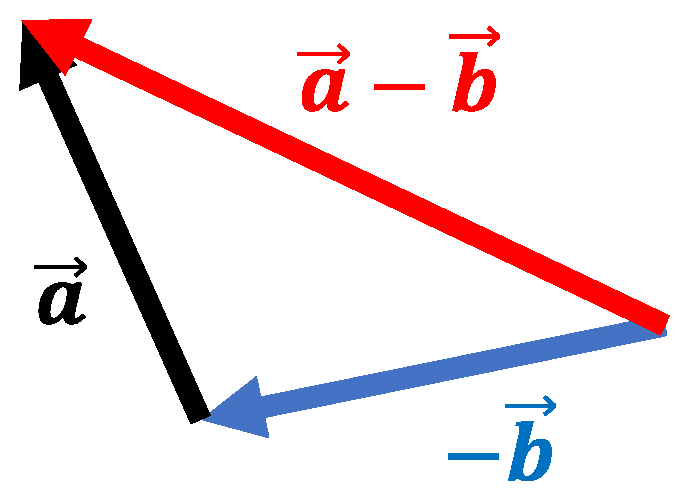
\includegraphics{img/vector_hikizan1.eps}
                        }
                    \end{center}
                    \caption{ベクトルの引き算1}
                    \label{fig:vector_hikizan1}
                \end{minipage}

                \begin{minipage}{0.45\hsize}
                    \begin{center}
                        \resizebox{0.7\hsize}{!}{
                        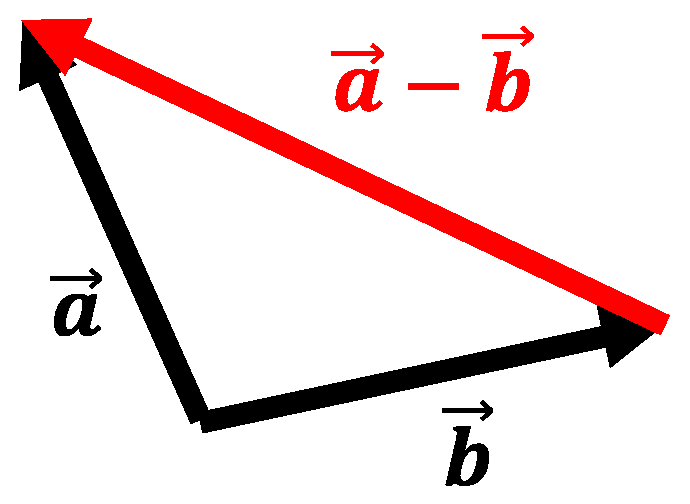
\includegraphics{img/vector_hikizan2.eps}
                        }
                    \end{center}
                    \caption{ベクトルの引き算2}
                    \label{fig:vector_hikizan2}
                \end{minipage}


            \end{tabular}
        \end{center}

    \end{figure}



    \subsection{積算}
    結論からいうとベクトル同士の掛け算はできない.と言ってしまうと残念な話であるが掛け算のような計算を導入することで対処する.

    まずはベクトルと定数の掛け算を考える.ベクトルの定数倍は大きさのみに作用する.$k\vec{a}$は図\ref{fig:vector_tesubai1}のような状態となる.負の数であれば逆向きになることもあわせて理解しよう(図\ref{fig:vector_tesubai2}).
    %

    \begin{figure}[htbp]
        \begin{center}
            \begin{tabular}{c}

                \begin{minipage}{0.45\hsize}
                    \begin{center}
                        \resizebox{!}{3cm}{
                        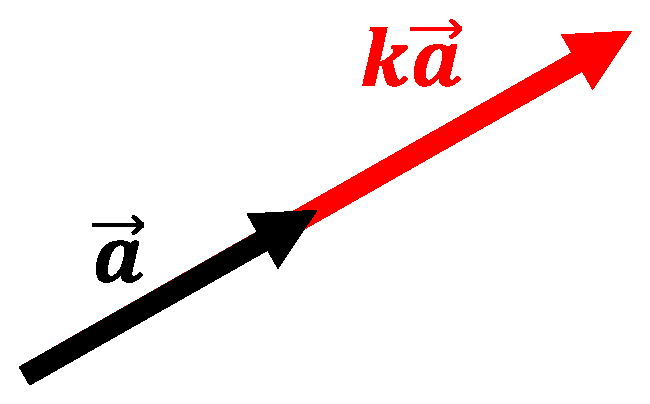
\includegraphics{img/vector_tesubai1.eps}
                        }
                    \end{center}
                    \caption{ベクトルの定数倍1}
                    \label{fig:vector_tesubai1}
                \end{minipage}

                \begin{minipage}{0.45\hsize}
                    \begin{center}
                        \resizebox{!}{3cm}{
                        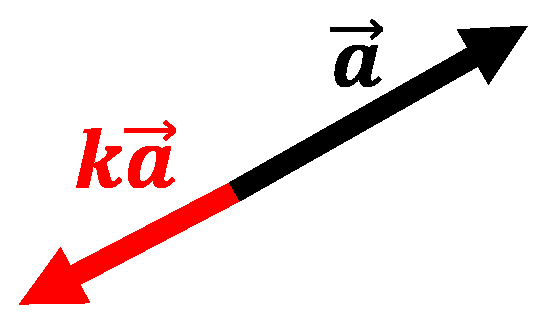
\includegraphics{img/vector_tesubai2.eps}
                        }
                    \end{center}
                    \caption{ベクトルの定数倍2}
                    \label{fig:vector_tesubai2}
                \end{minipage}


            \end{tabular}
        \end{center}

    \end{figure}


    次はベクトル同士の掛け算のような計算,すなわち内積を考える.内積の計算に求められるのは普通の計算で成立する次のような性質だ.
    \begin{enumerate}
        \item 定数倍
        \[
        (ka)\cdot b=k(a\cdot b)
        \]
        \item 交換の法則
        \[
        a\cdot b=b\cdot a
        \]
        \item 分配・結合の法則
        \[
        a\cdot(b+c)=a\cdot b + a\cdot c
        \]
    \end{enumerate}

    これを達成できるように内積を定める.図\ref{fig:vector_naiseki1}のような2つのベクトル$\vec{x},\vec{y}$に対して,
    \begin{equation}
        \vec{x}\cdot\vec{y}=|\vec{x}||\vec{y}|\cos\theta
        \label{eq:def_naiseki}
    \end{equation}
    と内積を定義する.
    %
    \begin{figure}[htbp]
        \begin{center}
            \resizebox{!}{3.5cm}{
            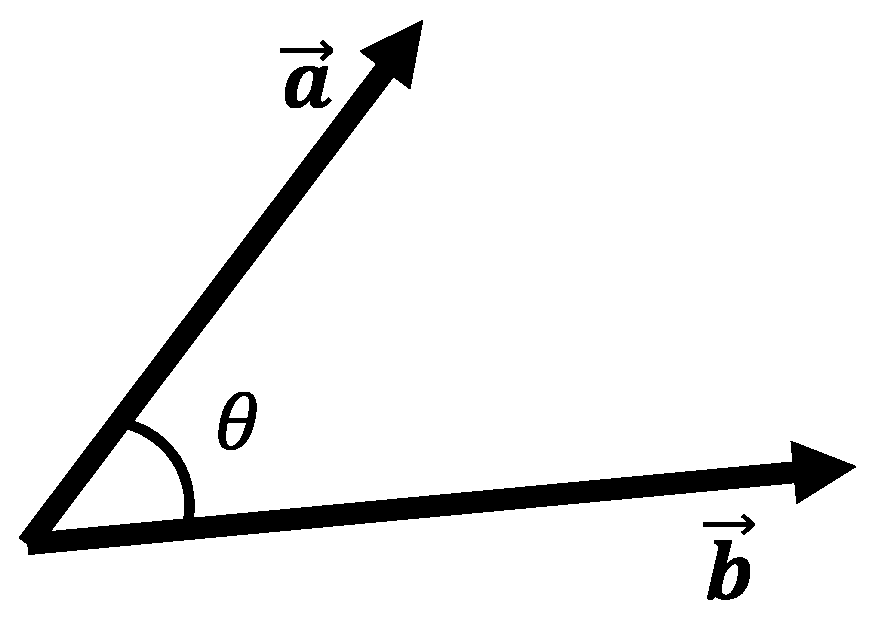
\includegraphics{img/vector_naiseki1.eps}
            }
        \end{center}
        \caption{内積}
        \label{fig:vector_naiseki1}
    \end{figure}

    図形的な理解をすると次のようになる(図\ref{fig:vector_naiseki2}).始点を共有している2つのベクトルにおいて,一方のベクトルの終点から他方のベクトルへ垂線をおろす.垂線の足とベクトルの始点との距離は図においては$|\vec{x}|\cos\theta$となる.これと垂線を下した先のベクトルの大きさ$|\vec{y}|$との積が内積の図形的な理解である.
    %
    \begin{figure}[htbp]
        \begin{center}
            \resizebox{!}{4cm}{
            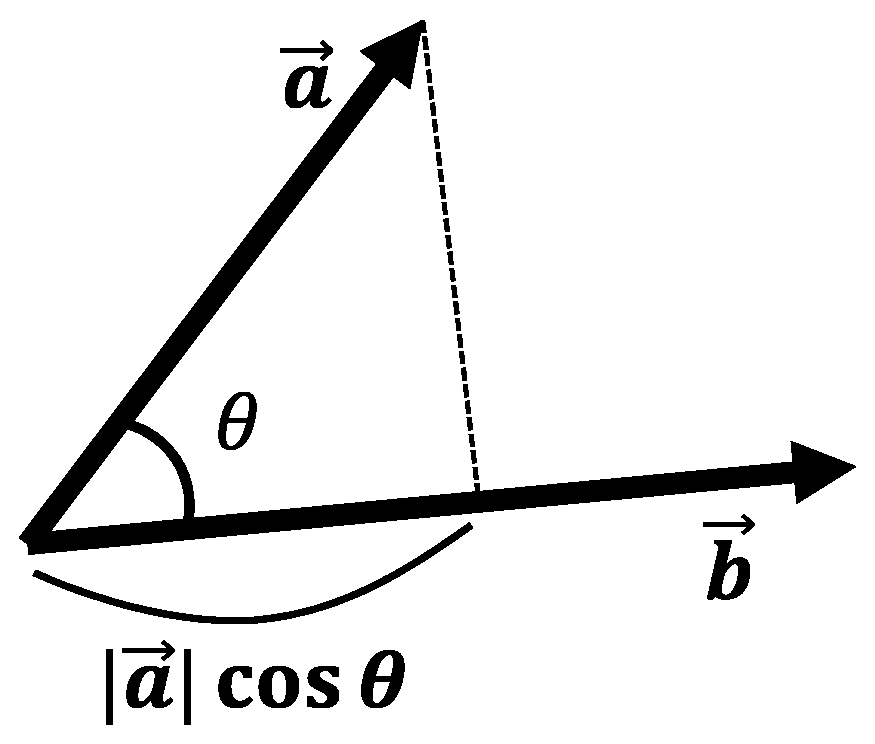
\includegraphics{img/vector_naiseki2.eps}
            }
        \end{center}
        \caption{内積の図形的理解}
        \label{fig:vector_naiseki2}
    \end{figure}




    内積に求められるのは先に挙げた性質と$\vec{x},\vec{y}$の持つ関係だ.$\cos\theta$となっているのは2つのベクトルのなす角が$0\leq\theta\leq\pi$であることからだ.$\sin\theta$では同じ値が2回出てしまう\footnote{$\sin x=\sin (\pi -x)$であることを言っている.}.これで内積は2つのベクトルの大きさと向きの2つの性質を合わせたものになっていることがわかる.

    ここからは内積が先に挙げた3つの性質を満たしているかを確認する内容だ.興味がなければ読み飛ばしてほしい.
    \begin{description}
        \item[定数倍] 定数$c>0$をとる.
        \begin{eqnarray*}
            (c\vec{x})\cdot(\vec{y})&=&|c\vec{x}||\vec{y}|\cos\theta\\
            &=&|c||\vec{x}||\vec{y}|\cos\theta\\
            &=&c(\vec{x}\cdot\vec{y})
        \end{eqnarray*}
        となる.次は$c<0$のとき
        \begin{eqnarray*}
            (c\vec{x})\cdot(\vec{y})&=& \{(-c)(-\vec{x})\}\cdot\vec{y}\\
            &=& |(-c)(-\vec{x})||\vec{y}|\cos(\pi-\theta)\\
            &=&-c|\vec{x}||\vec{y}|(-\cos\theta)\\
            &=&c(\vec{x}\cdot\vec{y})
        \end{eqnarray*}
        となり,定数倍の性質は満たす.図は後半の参考の図\ref{fig:vector_naiseki_tesubai}だ.
        %
        \begin{figure}[htbp]
            \begin{center}
                \resizebox{!}{4cm}{
                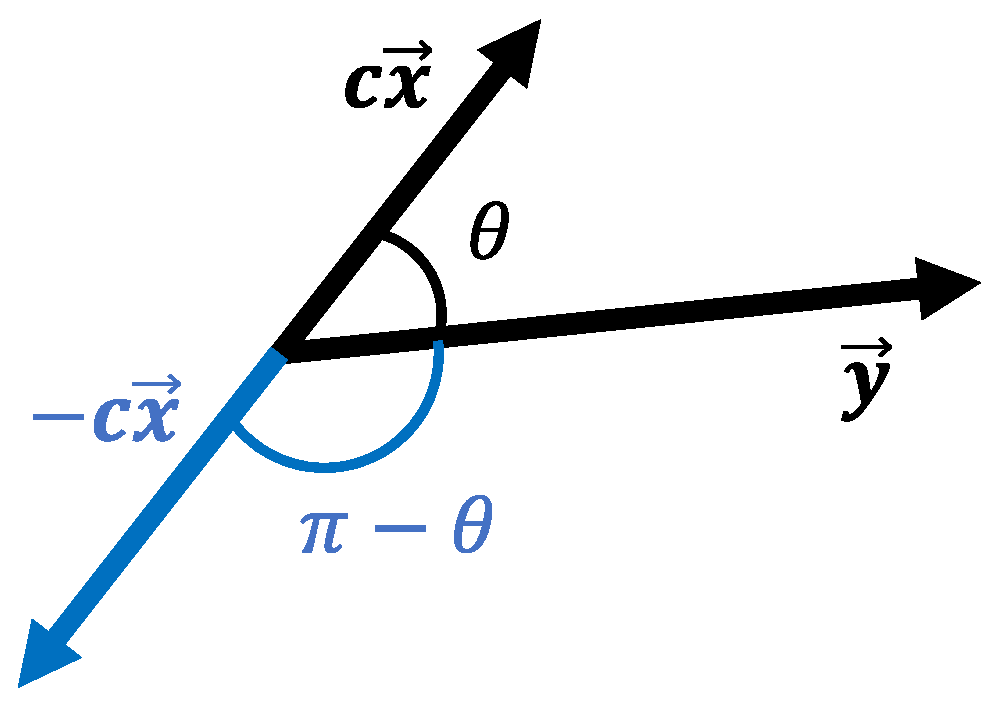
\includegraphics{img/vector_naiseki_tesubai.eps}
                }
            \end{center}
            \caption{内積の定数倍}
            \label{fig:vector_naiseki_tesubai}
        \end{figure}
        \item[交換の法則] 定義の式からも交換が可能であることは明らかだ.
        \[
        \vec{x}\cdot\vec{y}=|\vec{x}||\vec{y}|\cos\theta=|\vec{y}||\vec{x}|\cos\theta=\vec{y}\cdot\vec{x}
        \]
        \item[分配・結合の法則] 図\ref{fig:vector_naiseki_ketugo}の3つのベクトルから$(\vec{x}+\vec{y})\cdot\vec{z}$を考える.
        図\ref{fig:vector_naiseki_ketugo}から
        \[
        |\vec{x}+\vec{y}|\cos\theta= |\vec{x}|\cos\alpha +|\vec{y}|\cos\beta
        \]
        がわかるので,ここから
        \begin{eqnarray*}
            &|\vec{x}+\vec{y}||\vec{z}|\cos\theta= |\vec{x}||\vec{z}|\cos\alpha +|\vec{y}||\vec{z}|\cos\beta &\\
            &\Rightarrow (\vec{x}+\vec{y})\cdot\vec{z} =\vec{x}\cdot\vec{z} + \vec{y}\cdot\vec{z} &
        \end{eqnarray*}
        が計算される.
        %
        \begin{figure}[htbp]
            \begin{center}
                \resizebox{!}{6cm}{
                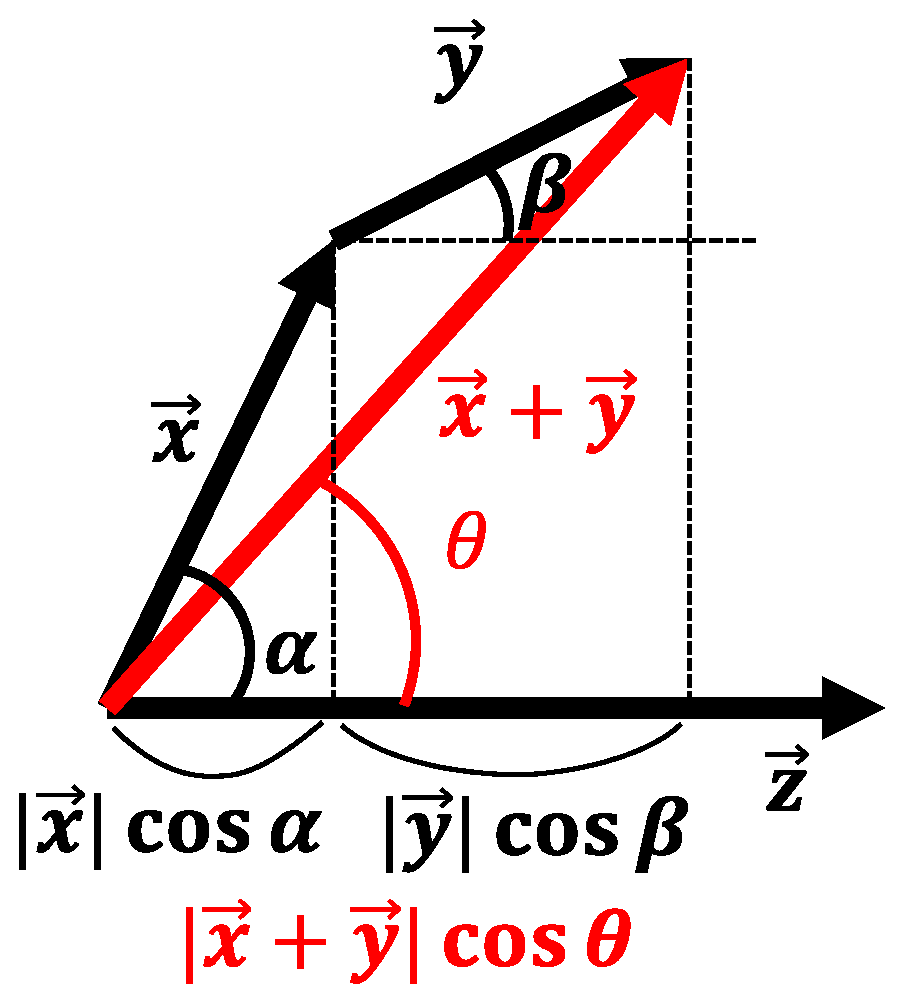
\includegraphics{img/vector_naiseki_ketugo.eps}
                }
            \end{center}
            \caption{結合法則}
            \label{fig:vector_naiseki_ketugo}
        \end{figure}

    \end{description}

    \subsection{2つのベクトルの関係}
    内積の定義式である式(\ref{eq:def_naiseki})から内積$\vec{a}\cdot\vec{b}$に次のことがわかる.
    \begin{eqnarray*}
        \theta =90^\circ=\frac{\pi}{2}&&\\
        &&\Rightarrow \vec{a}\cdot\vec{b} =0\\
        \theta = 0&&\\
        &&\Rightarrow \vec{a}\cdot\vec{b} = |\vec{a}||\vec{b}|
    \end{eqnarray*}
    これは$\cos\theta$の値のうち,特徴的なものから得られる関係だ.ここから次の同値関係がわかる.
    \begin{screen}
        \veczero ではない2つのベクトル\veca ,\vecb において$\vec{a}\cdot\vec{b}=0$であることと$\vec{a}\perp\vec{b}$であることは同値.

        数学的な式に直すと
        \[
        \vec{a},\vec{b}\neq\vec{0},\mmm\vec{a}\cdot\vec{b}=0\mmm\Leftrightarrow\mmm
        \vec{a}\perp\vec{b}
        \]
        と表される.

        この同値関係で重要なのは内積が0であることだけでは,2つのベクトルが垂直なのかがわからないところだ.\veczero であるときも内積は0となることに注意しよう.
    \end{screen}
    \begin{screen}
        \veca を2つで内積をとるとその値は\veca の大きさの2乗となり,${\vec{a}}^2$とは書かない.
        \[
        \vec{a}\cdot\vec{a}=|\vec{a}|^2
        \]
        これは簡単な式で取り上げる必要性もそれほど大きくないかもしれない.しかし,問題を解く上では頻出の関係なのであえて示す.
    \end{screen}

    次に平行な2つのベクトルを考える.これは2つのベクトルのなす角が0または$\pi$であるときだ.このような2つのベクトル\vecx ,\vecy に対しては次の関係が成り立つ.
    \[
    \vec{x}//\vec{y}\mmm \Leftrightarrow\mmm k\vec{x}=\vec{y}\mmm(kは実数)
    \]
    これも当然の式といえる.

    以上の関係は\veca のようなベクトルを利用して計算するときに主に使う式である.それと同時に\veca のようなベクトルは"平行"と"垂直"の2つが関係するときに大きな威力を発揮することを示している.これは逆に平行や垂直といった条件のない問題ではやや計算が困難になるということなので解答の方針を考える際は1つの指標にしてほしい.


    \subsection{$\vec{a}$のようなベクトルの計算のまとめ}
    先までの内容で$\vec{a}$などと表記されるタイプのベクトルを文字式のように計算できることが分かった.足し算や引き算はいつものように計算し,掛け算の部分を$\vec{a}\cdot\vec{b}$のように内積で表現すればいいのだ.

    そして,最初に述べた"向き"は計算できないという問題を\veca のような表現のベクトルでは
    $\vec{a}\cdot\vec{b}$や$|\vec{a}+\vec{b}|^2$といったベクトルをスカラにしてしまう計算によって解決している.




% \end{document}
